\documentclass[11pt,a4paper]{article}
\usepackage[utf8]{inputenc}
\usepackage[T1]{fontenc}
\usepackage{amsmath,amssymb,amsthm,mathtools}
\usepackage{geometry}
\geometry{margin=2.5cm}
\usepackage{booktabs}
\usepackage{xcolor}
\usepackage{tikz}
\usetikzlibrary{arrows.meta}
\usepackage{enumitem}
\usepackage{array}
\usepackage{lmodern}
\usepackage{microtype}
\usepackage{listings}
\usepackage{url}
\usepackage{hyperref}
\hypersetup{
    colorlinks=true,
    linkcolor=blue!70!black,
    citecolor=red!70!black,
    urlcolor=blue!70!black
}

\lstset{
    basicstyle=\ttfamily\footnotesize,
    breaklines=true,
    frame=single,
    numbers=none,
    mathescape=true,
    backgroundcolor=\color{gray!5}
}

\newtheorem{theorem}{Theorem}[section]
\newtheorem{lemma}[theorem]{Lemma}
\newtheorem{proposition}[theorem]{Proposition}
\newtheorem{corollary}[theorem]{Corollary}
\theoremstyle{definition}
\newtheorem{definition}[theorem]{Definition}
\newtheorem{remark}[theorem]{Remark}

\newcommand{\dee}{\mathrm{d}}
\newcommand{\Nset}{\mathbb{N}}
\newcommand{\Zset}{\mathbb{Z}}
\newcommand{\Rset}{\mathbb{R}}
\newcommand{\Cfield}{\mathbb{C}}

\title{\textbf{Constructive Candidate Sequences and Cotangent Gram Matrix Benchmarks on the B\'aez-Duarte Affine Manifold in Lean~4}}

\author{\textbf{Qamar Munawer}\\[0.3em]
\small Brandenburg University of Technology Cottbus--Senftenberg}

\date{November 2026}

\begin{document}
\linespread{1.15}\selectfont
\emergencystretch=2.5em

\maketitle

\begin{abstract}
We present the Lean~4 formalization and $80$-digit numerical benchmark analysis of constructive coefficient sequences on the B\'aez-Duarte affine manifold $\mathcal{A}_N = \{c \in \Rset^N : D_1(c, N) = 0 \land D_0(c, N) = 2\}$. Formally, our module \texttt{MathlibPR\_\allowbreak ForwardCandidate.lean} proves unconditional determinant positivity $\Delta(N) > 0$ for all $N \ge 2$, constructs the closed-form Euclidean projection \texttt{projectAffine}, defines explicit mollified M\"obius, Selberg sieve, and Clay--Galerkin candidate families whose squared $L^2(0, 1)$ approximation error reduces identically to $1 - S_{\mathrm{cot}}(c, N)$ with zero external integral hypotheses, and proves an exact closed-form evaluation at $N = 4$ certifying $S_{\mathrm{cot}}(c^{(4)}, 4) = (\frac{119}{576} + \frac{54467}{389376\sqrt{3}})\pi$ and strictly positive $L^2$ distance. Empirically, $80$-decimal-digit benchmarks across $N \in \{4, 8, 16, 32, 64, 128, 256\}$ confirm strict positive definiteness throughout, identify an empirical logarithmic decay rate $E_{\mathrm{opt}}(N) \approx C(\ln N)^{-1.12135}$ ($R^2_{\log} = 0.99976$), and diagnose the spectral condition-number and boundary-amplification obstructions. Epistemic invariant: \texttt{NO\_RH\_PROOF = TRUE}; no unconditional resolution of the Riemann Hypothesis is claimed.
\end{abstract}

\section{Introduction and Affine Projection Framework}

In the B\'aez-Duarte reformulation~\cite{BaezDuarte2003} of the Nyman--Beurling criterion, the Riemann Hypothesis holds if and only if the constant function $\mathbf{1}$ can be approximated in $L^2(0, 1)$ by finite linear combinations $\sum_{k=1}^N c_k \{1/(kx)\}$. Building on our unconditional formalization of Vasyunin's cross-integral~\cite{Vasyunin1995} and rank-4 boundary collapse, every vector $c \in \Rset^N$ lying on the affine manifold
\begin{equation}\label{eq:AN_def}
\mathcal{A}_N = \left\{ c : \Nset \to \Rset \;\middle|\; D_1(c, N) = \sum_{k=1}^N \frac{c_k}{k} = 0 \;\land\; D_0(c, N) = \sum_{k=1}^N c_k = 2 \right\}
\end{equation}
satisfies the exact pure cotangent distance identity
\begin{equation}\label{eq:l2_scot}
\int_0^1 \left(1 - \sum_{k=1}^N c_k \left\{\frac{1}{kx}\right\}\right)^2 \dee x = 1 - S_{\mathrm{cot}}(c, N),
\end{equation}
where $S_{\mathrm{cot}}(c, N) = \frac{\pi}{2}\sum_{j,k=1}^N \frac{c_j c_k}{jk}(V(j, k) + V(k, j))$ and $V(a, b) = \sum_{m=1}^{a-1} \{mb/a\}\cot(\pi m/a)$.

To bridge structural reductions to concrete arithmetic sequences, we investigate constructive candidate families $c^{(N)} \in \mathcal{A}_N$ both formally in \texttt{MathlibPR\_\allowbreak ForwardCandidate.lean} ($909$ lines, verified solely under \texttt{[propext, Classical.choice, Quot.sound]}) and numerically at $80$ decimal digits precision in \texttt{explore\_\allowbreak forward\_\allowbreak weights.py}.

\paragraph{Geometric Intuition.}
In $L^2(0, 1)$, restricting coefficient vectors $c$ to the codimension-$2$ affine manifold $\mathcal{A}_N$ slices out a flat hyperplane cone along which all smooth and logarithmic boundary terms of Vasyunin's kernel cancel identically, so orthogonal projection via \texttt{projectAffine} becomes a pure Euclidean drop onto the cotangent contraction axis $1 - S_{\mathrm{cot}}(c, N)$. High-precision exploration on this affine cone reveals both why low-$N$ projections contract smoothly ($E_{\mathrm{opt}}(256) = 0.008243$) and where finite geometric intuition hits genuine spectral walls ($\kappa(G_{64}) = 11{,}555.80$ and $\det(U_4)^{-1} \approx 664.38\times$).

\paragraph{Epistemic Demarcation (\texttt{NO\_RH\_PROOF = TRUE}).}
All formal statements in Section~\ref{sec:candidates}--\ref{sec:N4} prove structural identities, membership in $\mathcal{A}_N$, exact finite-$N$ evaluations, or \emph{conditional} implications toward \texttt{RiemannHypothesis}. Neither the Lean~4 development nor the numerical benchmarks up to $N = 256$ establish $\lim_{N\to\infty} S_{\mathrm{cot}}(c^{(N)}, N) = 1$, and the Riemann Hypothesis remains an open conjecture.

\subsection{Two-Constraint Affine Projection and Determinant Positivity}

Given an arbitrary raw weight sequence $u : \Nset \to \Rset$, let
\begin{equation}
H(N) = \sum_{k=1}^N \frac{1}{k}, \qquad S_2(N) = \sum_{k=1}^N \frac{1}{k^2}, \qquad \Delta(N) = N S_2(N) - H(N)^2,
\end{equation}
formalized as \texttt{HSum}, \texttt{S2Sum}, and \texttt{DeltaDet}. Minimizing $\|c - u\|_2^2$ subject to $c \in \mathcal{A}_N$ produces the orthogonal Euclidean projection \texttt{projectAffine}:
\begin{equation}\label{eq:projectAffine}
c_k = (\text{\texttt{projectAffine}}\, u\, N)_k = u_k - \frac{\lambda_1(u, N)}{k} - \lambda_0(u, N) \qquad (1 \le k \le N),
\end{equation}
with explicit Lagrange multipliers
\begin{equation}
\lambda_1(u, N) = \frac{N U_1 - H(N)(U_0 - 2)}{\Delta(N)}, \qquad \lambda_0(u, N) = \frac{S_2(N)(U_0 - 2) - H(N) U_1}{\Delta(N)},
\end{equation}
where $U_1 = \sum_{k=1}^N u_k/k$ and $U_0 = \sum_{k=1}^N u_k$. Algebraic elimination in \texttt{projectAffine\_D1} and \texttt{projectAffine\_D0} shows $D_1(\text{\texttt{projectAffine}}\, u\, N, N) = 0$ and $D_0(\text{\texttt{projectAffine}}\, u\, N, N) = 2$ whenever $\Delta(N) \ne 0$.

To discharge $\Delta(N) \ne 0$ unconditionally for all $N \ge 2$, lemma \texttt{DeltaDet\_double\_sum\_eq} establishes the Lagrange Cauchy--Schwarz identity
\begin{equation}
2 \Delta(N) = \sum_{j=1}^N \sum_{k=1}^N \left(\frac{1}{j} - \frac{1}{k}\right)^2.
\end{equation}
For $N \ge 2$, isolating the strictly positive $(j, k) = (1, 2)$ summand $(1 - 1/2)^2 = 1/4$ gives unconditional positivity \texttt{DeltaDet\_pos}, \texttt{DeltaDet\_ne\_zero}, and \texttt{projectAffine\_mem\_A\_N\_uncond}:
\begin{lstlisting}
theorem DeltaDet_double_sum_eq (N : $\Nset$) :
    2 * DeltaDet N =
      $\sum$ j $\in$ Finset.Icc 1 N, $\sum$ k $\in$ Finset.Icc 1 N, ((1 : $\Rset$) / (j : $\Rset$) - (1 : $\Rset$) / (k : $\Rset$)) ^ 2

theorem DeltaDet_pos {N : $\Nset$} (hN : 2 $\le$ N) : 0 < DeltaDet N

theorem projectAffine_mem_A_N_uncond (u : $\Nset \to \Rset$) {N : $\Nset$} (hN : 2 $\le$ N) :
    D1 (projectAffine u N) N = 0 $\land$ D0 (projectAffine u N) N = 2
\end{lstlisting}

\section{Constructive Candidate Families and Unconditional Distance Bridge}\label{sec:candidates}

We formalize three explicit arithmetic candidate families on $\mathcal{A}_N$ inside \texttt{MathlibPR\_\allowbreak ForwardCandidate.lean}:
\begin{enumerate}[noitemsep]
  \item \textbf{Quadratic Mollified M\"obius (\texttt{cCandidateMobius}):} Using the M\"obius function $\mu(k)$, set
  \begin{align}
  \text{\texttt{mollifiedMobius}}(N, k) &= -\mu(k)\left(1 - \frac{k}{N}\right)^2, \\
  \text{\texttt{cCandidateMobius}}(N) &= \text{\texttt{projectAffine}}(\text{\texttt{mollifiedMobius}}\, N, N).
  \end{align}
  \item \textbf{Selberg Sieve Weight (\texttt{cCandidateSelberg}):} Set $\text{\texttt{selbergSieveWeights}}(N, k) = -\mu(k)\big(\ln(N/k)/\ln N\big)^2$ for $k < N$ and $0$ for $k = N$, projected via $\text{\texttt{cCandidateSelberg}}(N) = \text{\texttt{projectAffine}}(\text{\texttt{selbergSieveWeights}}\, N, N)$.
  \item \textbf{Clay--Galerkin Base-Plus-Ray (\texttt{clayGalerkinCandidate}):} Combining the canonical 4-point base vector \texttt{clayRank4Base} ($N \ge 4$) satisfying all four boundary moments $(D_0, D_0', D_1, D_1') = (2, 0, 0, 0)$ with the homogeneous cotangent ray \texttt{clayRank4GalerkinRay vasyuninGCot u N}, define
  \begin{equation}
  \text{\texttt{clayGalerkinCandidate}}(u, N, k) = \text{\texttt{clayRank4Base}}\, k + u_{\text{ray}}(k),
  \end{equation}
  where $u_{\text{ray}}(k) = \text{\texttt{clayRank4GalerkinRay}}\, \text{\texttt{vasyuninGCot}}\, u\, N\, k$.
\end{enumerate}

By \texttt{projectAffine\_mem\_A\_N\_uncond} (for $N \ge 2$) and \texttt{clayRank4Base\_mem\_A\_N} paired with homogeneous boundary preservation (for $N \ge 4$), all three families lie unconditionally in $\mathcal{A}_N$. Consequently, all smooth logarithmic and Euler--Mascheroni terms drop out identically via \texttt{affine\_l2\_dist\_eq\_one\_sub\_scot}, yielding exact distance reductions free of external integral or determinantal assumptions:
\begin{lstlisting}
theorem projectAffine_l2_dist_eq_one_sub_scot (u : $\Nset \to \Rset$) (N : $\Nset$) (h$\Delta$ : DeltaDet N $\ne$ 0) :
    ($\int$ x in (0 : $\Rset$)..1, (1 - $\sum$ k $\in$ Finset.Icc 1 N, projectAffine u N k * recipFractScaled k x) ^ 2) =
      1 - SCot vasyuninGCot (projectAffine u N) N

theorem clayGalerkinCandidate_l2_dist_eq_one_sub_scot (u : $\Nset \to \Rset$) {N : $\Nset$} (hN : 4 $\le$ N) :
    ($\int$ x in (0 : $\Rset$)..1, (1 - $\sum$ k $\in$ Finset.Icc 1 N, clayGalerkinCandidate u N k * recipFractScaled k x) ^ 2) =
      1 - SCot vasyuninGCot (clayGalerkinCandidate u N) N

theorem riemannHypothesis_of_cCandidateMobius_limit
    (h_limit : $\forall$ $\varepsilon$ > 0, $\exists$ N : $\Nset$, 2 $\le$ N $\land$ 1 - $\varepsilon$ < SCot vasyuninGCot (cCandidateMobius N) N) :
    RiemannHypothesis

theorem riemannHypothesis_of_cCandidateSelberg_limit
    (h_limit : $\forall$ $\varepsilon$ > 0, $\exists$ N : $\Nset$, 2 $\le$ N $\land$ 1 - $\varepsilon$ < SCot vasyuninGCot (cCandidateSelberg N) N) :
    RiemannHypothesis

theorem riemannHypothesis_of_clayGalerkin_limit (u : $\Nset \to \Rset$)
    (h_limit : $\forall$ $\varepsilon$ > 0, $\exists$ N : $\Nset$, 4 $\le$ N $\land$ 1 - $\varepsilon$ < SCot vasyuninGCot (clayGalerkinCandidate u N) N) :
    RiemannHypothesis
\end{lstlisting}
All theorems depend strictly on Lean~4's core foundational axioms \texttt{[propext, Classical.choice, Quot.sound]} (verified via \texttt{\#print axioms}), with zero \texttt{sorry}.

\section{Exact Closed-Form Certification at \texorpdfstring{$N = 4$}{N = 4} in Lean~4}\label{sec:N4}

To provide a completely algebraic sanity check of both the Lagrange projection and the cotangent quadratic form, \texttt{MathlibPR\_\allowbreak ForwardCandidate.lean} evaluates \texttt{cCandidateMobius 4} in exact arithmetic. Direct summation certifies \texttt{HSum\_four : HSum 4 = 25 / 12}, \texttt{S2Sum\_four : S2Sum 4 = 205 / 144}, and \texttt{DeltaDet\_four : DeltaDet 4 = 65 / 48}. Using $\mu(1) = 1$, $\mu(2) = -1$, $\mu(3) = -1$, and $\mu(4) = 0$ gives (\texttt{mollifiedMobius\_four\_eval}):
\begin{equation}
u(1) = -\frac{9}{16}, \qquad u(2) = \frac{1}{4}, \qquad u(3) = \frac{1}{16}, \qquad u(4) = 0,
\end{equation}
with Lagrange multipliers $\lambda_1 = 29/13$ and $\lambda_0 = -269/156$, yielding the exact projected coefficients (\texttt{cCandidateMobius\_four\_eval}):
\begin{equation}
c_1^{(4)} = -\frac{667}{624}, \qquad c_2^{(4)} = \frac{67}{78}, \qquad c_3^{(4)} = \frac{217}{208}, \qquad c_4^{(4)} = \frac{7}{6}.
\end{equation}
One checks immediately that $D_1 = -667/624 + 67/156 + 217/624 + 7/24 = 0$ and $D_0 = (-667 + 536 + 651 + 728)/624 = 2$.

Evaluating the off-diagonal Vasyunin cotangent entries for $1 \le j < k \le 4$ via $\cot(\pi/3) = 1/\sqrt{3}$, $\cot(2\pi/3) = -1/\sqrt{3}$, $\cot(\pi/4) = 1$, and $\cot(3\pi/4) = -1$ gives
\begin{align}
g_{1,2}^{\mathrm{cot}} &= 0, &
g_{1,3}^{\mathrm{cot}} &= \frac{\pi}{18\sqrt{3}}, &
g_{1,4}^{\mathrm{cot}} &= \frac{\pi}{16}, \\
g_{2,3}^{\mathrm{cot}} &= -\frac{\pi}{36\sqrt{3}}, &
g_{2,4}^{\mathrm{cot}} &= 0, &
g_{3,4}^{\mathrm{cot}} &= \frac{\pi}{72\sqrt{3}} - \frac{\pi}{48},
\end{align}
and expanding $S_{\mathrm{cot}}(c^{(4)}, 4) = -\sum_{j,k=1}^4 c_j^{(4)} c_k^{(4)} g_{j,k}^{\mathrm{cot}}$ gives the exact Lean~4 theorem \texttt{SCot\_\allowbreak cCandidateMobius\_\allowbreak four\_\allowbreak eq}, continuous $L^2$ identity \texttt{cCandidateMobius\_\allowbreak four\_\allowbreak l2\_\allowbreak dist\_\allowbreak eq}, and strict positivity witness \texttt{cCandidateMobius\_\allowbreak four\_\allowbreak l2\_\allowbreak dist\_\allowbreak pos} (using $\sqrt{3} > 1.732$ and $\pi < 3.1416$):
\begin{lstlisting}
theorem SCot_cCandidateMobius_four_eq :
    SCot vasyuninGCot (cCandidateMobius 4) 4 =
      ((119 : $\Rset$) / 576 + 54467 / (389376 * Real.sqrt 3)) * Real.pi

theorem cCandidateMobius_four_l2_dist_eq :
    ($\int$ x in (0 : $\Rset$)..1,
      (1 - $\sum$ k $\in$ Finset.Icc 1 4, cCandidateMobius 4 k * recipFractScaled k x) ^ 2) =
      1 - ((119 : $\Rset$) / 576 + 54467 / (389376 * Real.sqrt 3)) * Real.pi

theorem cCandidateMobius_four_l2_dist_pos :
    0 < ($\int$ x in (0 : $\Rset$)..1,
      (1 - $\sum$ k $\in$ Finset.Icc 1 4, cCandidateMobius 4 k * recipFractScaled k x) ^ 2)
\end{lstlisting}
Numerically, $S_{\mathrm{cot}}(c^{(4)}, 4) \approx 0.9027636254$ and the continuous $L^2(0, 1)$ squared error is $E_{\mathrm{cot}}(4) = 1 - S_{\mathrm{cot}}(c^{(4)}, 4) \approx 0.0972363746 > 0$, matching the $80$-digit benchmark in Section~\ref{sec:benchmark} to all printed digits.

\subsection{Affine Cotangent Improvement Identity and Suboptimality of M\"obius at \texorpdfstring{$N = 4$}{N = 4}}

For any two vectors $c, c' \in \mathcal{A}_N$, subtracting the pure cotangent distance identity~\eqref{eq:l2_scot} cancels all baseline constants and yields the exact comparison law (\texttt{l2\_\allowbreak dist\_\allowbreak sub\_\allowbreak eq\_\allowbreak scot\_\allowbreak sub} and \texttt{l2\_\allowbreak dist\_\allowbreak lt\_\allowbreak iff\_\allowbreak scot\_\allowbreak gt}):
\begin{equation}
\int_0^1 \!\left(1 - \sum_{k=1}^N c'_k \left\{\frac{1}{kx}\right\}\right)^{\!2}\!\dee x
- \int_0^1 \!\left(1 - \sum_{k=1}^N c_k \left\{\frac{1}{kx}\right\}\right)^{\!2}\!\dee x
= S_{\mathrm{cot}}(c, N) - S_{\mathrm{cot}}(c', N),
\end{equation}
so $c'$ strictly improves upon $c$ in $L^2(0, 1)$ if and only if $S_{\mathrm{cot}}(c, N) < S_{\mathrm{cot}}(c', N)$.

To demonstrate unconditionally that the classical quadratic mollified M\"obius vector \texttt{cCandidateMobius 4} is not optimal on $\mathcal{A}_4$, we extract the simple rational variational vector \texttt{cVariationalFour}:
\begin{equation}
c_{\mathrm{var},1}^{(4)} = -\frac{21}{20}, \qquad
c_{\mathrm{var},2}^{(4)} = \frac{3}{4}, \qquad
c_{\mathrm{var},3}^{(4)} = \frac{6}{5}, \qquad
c_{\mathrm{var},4}^{(4)} = \frac{11}{10},
\end{equation}
chosen near the unconstrained KKT optimum on $\mathcal{A}_4$. Exact rational arithmetic verifies \texttt{cVariationalFour\_\allowbreak mem\_\allowbreak A\_\allowbreak N} ($D_1 = 0$, $D_0 = 2$) and evaluates $S_{\mathrm{cot}}$ in closed form as
\begin{equation}
S_{\mathrm{cot}}\big(c_{\mathrm{var}}^{(4)}, 4\big)
= \left(\frac{319}{1600} + \frac{23}{150\sqrt{3}}\right)\pi \approx 0.9044709378
\quad \big(E_{\mathrm{cot}}(4) \approx 0.0955290622\big),
\end{equation}
capturing over $92\%$ of the improvement up to the full KKT optimum ($S_{\mathrm{cot}} \approx 0.9046063682$). Bounding $1.732 < \sqrt{3} < 1.7321$ and $\pi < 3.1416$ in Lean~4 proves unconditionally that $c_{\mathrm{var}}^{(4)}$ strictly beats \texttt{cCandidateMobius 4} while preserving positive $L^2$ error (\texttt{UpstreamPR\_\allowbreak 3H\_\allowbreak VariationalOptimumFour.lean}):
\begin{lstlisting}
theorem l2_dist_lt_iff_scot_gt {N : $\Nset$} (c c' : $\Nset \to \Rset$)
    (hc1 : D1 c N = 0) (hc0 : D0 c N = 2) (hc1' : D1 c' N = 0) (hc0' : D0 c' N = 2) :
    ($\int$ x in (0 : $\Rset$)..1, (1 - $\sum$ k $\in$ Finset.Icc 1 N, c' k * recipFractScaled k x) ^ 2) <
      ($\int$ x in (0 : $\Rset$)..1, (1 - $\sum$ k $\in$ Finset.Icc 1 N, c k * recipFractScaled k x) ^ 2) $\leftrightarrow$
      SCot vasyuninGCot c N < SCot vasyuninGCot c' N

theorem SCot_cVariationalFour_eq :
    SCot vasyuninGCot cVariationalFour 4 =
      ((319 : $\Rset$) / 1600 + 23 / (150 * Real.sqrt 3)) * Real.pi

theorem SCot_cCandidateMobius_four_lt_cVariationalFour :
    SCot vasyuninGCot (cCandidateMobius 4) 4 < SCot vasyuninGCot cVariationalFour 4

theorem l2_dist_cVariationalFour_lt_cCandidateMobius_four :
    ($\int$ x in (0 : $\Rset$)..1,
      (1 - $\sum$ k $\in$ Finset.Icc 1 4, cVariationalFour k * recipFractScaled k x) ^ 2) <
      ($\int$ x in (0 : $\Rset$)..1,
        (1 - $\sum$ k $\in$ Finset.Icc 1 4, cCandidateMobius 4 k * recipFractScaled k x) ^ 2)

theorem cVariationalFour_l2_dist_pos :
    0 < ($\int$ x in (0 : $\Rset$)..1,
      (1 - $\sum$ k $\in$ Finset.Icc 1 4, cVariationalFour k * recipFractScaled k x) ^ 2)
\end{lstlisting}

\subsection{Minimum-Norm Base Point and Orthogonal Tangent Decomposition of \texorpdfstring{$\mathcal{A}_N$}{A\_N}}

Projecting the zero seed via~\eqref{eq:projectAffine} isolates the unique minimum-$\ell^2$-norm element $c_{\min}^{(N)} := \texttt{projectAffine}\;(\lambda \_ \Rightarrow 0)\;N$ on $\mathcal{A}_N$ (\texttt{UpstreamPR\_\allowbreak 4B\_\allowbreak AffineOrthogonalDecomp.lean}):
\begin{equation}
c_{\min,k}^{(N)} = \frac{2 S_2(N) - 2 H(N) / k}{\Delta(N)}, \qquad
\sum_{k=1}^N \big(c_{\min,k}^{(N)}\big)^2 = \frac{4 S_2(N)}{\Delta(N)}.
\end{equation}
Because $c_{\min}^{(N)}$ lies in $\operatorname{span}\{1, 1/k\}$, it is $\ell^2$-orthogonal to every vector $h$ in the homogeneous tangent subspace $\mathcal{A}_N^0 = \{h : D_1(h, N) = 0 \land D_0(h, N) = 0\}$ (\texttt{cMinNorm\_\allowbreak inner\_\allowbreak eq\_\allowbreak zero}). Consequently, every $c \in \mathcal{A}_N$ ($N \ge 2$) admits the exact Pythagorean decomposition (\texttt{norm\_\allowbreak sq\_\allowbreak eq\_\allowbreak cMinNorm\_\allowbreak add\_\allowbreak sub\_\allowbreak sq}):
\begin{equation}
\sum_{k=1}^N c_k^2 = \frac{4 S_2(N)}{\Delta(N)} + \sum_{k=1}^N \big(c_k - c_{\min,k}^{(N)}\big)^2
\;\ge\; \frac{4 S_2(N)}{\Delta(N)},
\end{equation}
with exact benchmark $\sum_{k=1}^4 (c_{\min,k}^{(4)})^2 = 164/39 \approx 4.205128$ (\texttt{cMinNorm\_\allowbreak norm\_\allowbreak sq\_\allowbreak four}). This avoids the ill-conditioned $4$-constraint $U_4$ matrix entirely and isolates $\mathcal{A}_N^0$ as the natural unconstrained search space for variational optimization.

\subsection{Determinant-Free Base Anchor and Harmonic Wavelet Basis of \texorpdfstring{$\mathcal{A}_N$}{A\_N}}

While $c_{\min}^{(N)}$ requires $\Delta(N)$, $\mathcal{A}_N$ admits an exact determinant-free parameterization (\texttt{UpstreamPR\_\allowbreak 4C\_\allowbreak HarmonicWaveletBasis.lean}) anchored at the $2$-point vector $c_{\mathrm{anchor}} = (-2, 4, 0, \dots)$ (\texttt{cBaseAnchor}). Since all Vasyunin cotangent interactions on $\{1, 2\}$ vanish identically, \texttt{SCot\_\allowbreak cBaseAnchor\_\allowbreak eq\_\allowbreak zero} certifies $S_{\mathrm{cot}}(c_{\mathrm{anchor}}, N) = 0$ and baseline error $E(c_{\mathrm{anchor}}, N) = 1$ (\texttt{cBaseAnchor\_\allowbreak l2\_\allowbreak dist\_\allowbreak eq\_\allowbreak one}). Every $3$-point harmonic wavelet
\begin{equation}
w_k^{(m)} = \begin{cases}
m, & k = m, \\
-2(m + 1), & k = m + 1, \\
m + 2, & k = m + 2, \\
0, & \text{otherwise}
\end{cases}
\end{equation}
($1 \le m \le N - 2$) satisfies $D_1(w^{(m)}, N) = 1 - 2 + 1 = 0$ and $D_0(w^{(m)}, N) = m - 2(m+1) + (m+2) = 0$ without divisions (\texttt{harmonicWavelet\_\allowbreak mem\_\allowbreak tangent}), so $c_{\mathrm{anchor}} + \sum_m \alpha_m w^{(m)} \in \mathcal{A}_N$ unconditionally (\texttt{cBaseAnchor\_\allowbreak add\_\allowbreak smul\_\allowbreak wavelet\_\allowbreak mem\_\allowbreak A\_\allowbreak N}). In particular, \texttt{cVariationalFour} decomposes exactly in this wavelet basis (\texttt{cVariationalFour\_\allowbreak eq\_\allowbreak wavelet\_\allowbreak decomp}):
\begin{equation}
c_{\mathrm{var}}^{(4)} = c_{\mathrm{anchor}} + \frac{19}{20} w^{(1)} + \frac{11}{40} w^{(2)}.
\end{equation}

Expanding $c = c_{\mathrm{anchor}} + h$ directly inside $S_{\mathrm{cot}}$ (\texttt{UpstreamPR\_\allowbreak 4D\_\allowbreak Wavelet\allowbreak Cotangent\allowbreak Stencil.lean}) eliminates $S_{\mathrm{cot}}(c_{\mathrm{anchor}}, N) = 0$ and isolates a linear $1/k$-weighted contrast sum (\texttt{SCot\_\allowbreak cBaseAnchor\_\allowbreak add\_\allowbreak eq}), where $\delta_{\mathrm{cot}}(k) = V(k, 2) - V(k, 1)$ (\texttt{deltaCot}):
\begin{equation}
S_{\mathrm{cot}}(c_{\mathrm{anchor}} + h, N) = S_{\mathrm{cot}}(h, N) + 2\pi \sum_{k=1}^N \frac{h_k}{k}\,\delta_{\mathrm{cot}}(k).
\end{equation}
Because multiplying $F(k)/k$ by $w_k^{(m)}$ cancels the $1/k$ denominator identically into the unweighted second difference $\Delta^2 F(m) = F(m) - 2F(m+1) + F(m+2)$ (\texttt{harmonicWavelet\_\allowbreak div\_\allowbreak sum\_\allowbreak eq\_\allowbreak second\_\allowbreak diff}), any single-wavelet ray $c_t = c_{\mathrm{anchor}} + t w^{(m)}$ reduces to the scalar quadratic stencil law (\texttt{SCot\_\allowbreak cBaseAnchor\_\allowbreak add\_\allowbreak smul\_\allowbreak wavelet\_\allowbreak eq}):
\begin{equation}
S_{\mathrm{cot}}(c_{\mathrm{anchor}} + t w^{(m)}, N) = t^2 S_{\mathrm{cot}}(w^{(m)}, N) + 2\pi t \big(\delta_{\mathrm{cot}}(m) - 2\delta_{\mathrm{cot}}(m+1) + \delta_{\mathrm{cot}}(m+2)\big).
\end{equation}

On the homogeneous tangent subspace $\mathcal{A}_N^0$ ($D_1(h, N) = 0 \land D_0(h, N) = 0$), the smooth Vasyunin kernel vanishes identically (\texttt{sum\_\allowbreak GSmooth\_\allowbreak eq\_\allowbreak zero\_\allowbreak of\_\allowbreak mem\_\allowbreak tangent}), yielding an exact Hilbert-space isometry (\texttt{UpstreamPR\_\allowbreak 4E\_\allowbreak Tangent\allowbreak Cotangent\allowbreak Positivity.lean}, \texttt{tangent\_\allowbreak l2\_\allowbreak norm\_\allowbreak sq\_\allowbreak eq\_\allowbreak qcot}):
\begin{equation}
\int_0^1 \!\left(\sum_{k=1}^N h_k \left\{\frac{1}{kx}\right\}\right)^{\!2}\!\dee x
= Q_{\mathrm{cot}}(h, N) \ge 0,
\qquad S_{\mathrm{cot}}(h, N) \le 0,
\end{equation}
giving unconditional positive semidefiniteness (\texttt{QCot\_\allowbreak nonneg\_\allowbreak of\_\allowbreak mem\_\allowbreak tangent}, \texttt{SCot\_\allowbreak nonpos\_\allowbreak of\_\allowbreak mem\_\allowbreak tangent}). Evaluating the first harmonic wavelet $w^{(1)} = (1, -4, 3)$ at $N = 3$ certifies $Q_{\mathrm{cot}}(w^{(1)}, 3) = \|w^{(1)}\|_{L^2}^2 = \pi/\sqrt{3}$ (\texttt{QCot\_\allowbreak harmonic\allowbreak Wavelet\_\allowbreak one\_\allowbreak eq}, \texttt{harmonic\allowbreak Wavelet\_\allowbreak one\_\allowbreak l2\_\allowbreak norm\_\allowbreak sq\_\allowbreak eq}), so the ray $c_{\mathrm{anchor}} + t w^{(1)}$ maximizes $S_{\mathrm{cot}}$ at step size $t = 2/3$ with exact $N = 3$ variational optimum (\texttt{SCot\_\allowbreak cBaseAnchor\_\allowbreak add\_\allowbreak two\_\allowbreak thirds\_\allowbreak wavelet\_\allowbreak one\_\allowbreak eq}):
\begin{equation}
S_{\mathrm{cot}}\!\left(c_{\mathrm{anchor}} + \frac{2}{3} w^{(1)}, 3\right) = \frac{4\pi}{9\sqrt{3}}.
\end{equation}

Generalizing along arbitrary tangent rays $c_{\mathrm{anchor}} + t h$ with $h \in \mathcal{A}_N^0$ (\texttt{UpstreamPR\_\allowbreak 4F\_\allowbreak Tangent\allowbreak Rayleigh\allowbreak Quotient.lean}) via the linear cotangent drive $\mathcal{L}_{\mathrm{cot}}(h, N) := \sum_{k=1}^N \frac{h_k}{k}\delta_{\mathrm{cot}}(k)$ (\texttt{linearCotDrive}), optimal step $t^\star = \pi \mathcal{L}_{\mathrm{cot}}(h, N) / Q_{\mathrm{cot}}(h, N)$ (\texttt{optTangentStep}), and scale-invariant tangent Rayleigh quotient
\begin{equation}
\mathcal{R}_{\mathrm{cot}}(h, N) := \frac{\big(\pi\,\mathcal{L}_{\mathrm{cot}}(h, N)\big)^2}{Q_{\mathrm{cot}}(h, N)}
\end{equation}
(\texttt{tangentRayleighQuotient}) yields the exact completing-the-square law (\texttt{SCot\_\allowbreak cBaseAnchor\_\allowbreak add\_\allowbreak smul\_\allowbreak eq\_\allowbreak rayleigh\_\allowbreak sub\_\allowbreak sq}):
\begin{equation}
S_{\mathrm{cot}}(c_{\mathrm{anchor}} + t h, N) = \mathcal{R}_{\mathrm{cot}}(h, N) - Q_{\mathrm{cot}}(h, N)\,(t - t^\star)^2,
\end{equation}
attained at $t = t^\star$ (\texttt{SCot\_\allowbreak cBaseAnchor\_\allowbreak add\_\allowbreak optTangentStep\_\allowbreak eq}). Combining this identity with $S_{\mathrm{cot}}(c, N) \le 1$ proves the unconditional cotangent Cauchy--Schwarz inequality $\big(\pi\,\mathcal{L}_{\mathrm{cot}}(h, N)\big)^2 \le Q_{\mathrm{cot}}(h, N)$ (\texttt{sq\_\allowbreak linearCotDrive\_\allowbreak le\_\allowbreak qcot}) and the scale-invariant ceiling $\mathcal{R}_{\mathrm{cot}}(h, N) \le 1$ for all $N \ge 2$ and $h \in \mathcal{A}_N^0$ (\texttt{tangentRayleighQuotient\_\allowbreak le\_\allowbreak one}). \noindent In particular, along $w^{(1)}$ at $N = 3$ this establishes the global bound $S_{\mathrm{cot}}(c_{\mathrm{anchor}} + t w^{(1)}, 3) = \frac{4\pi}{9\sqrt{3}} - \frac{\pi}{\sqrt{3}}(t - \tfrac{2}{3})^2 \le \frac{4\pi}{9\sqrt{3}}$ for every $t \in \mathbb{R}$ (\texttt{SCot\_\allowbreak cBaseAnchor\_\allowbreak add\_\allowbreak smul\_\allowbreak wavelet\_\allowbreak one\_\allowbreak eq\_\allowbreak completing\_\allowbreak sq}, \texttt{SCot\_\allowbreak cBaseAnchor\_\allowbreak add\_\allowbreak smul\_\allowbreak wavelet\_\allowbreak one\_\allowbreak le}).

At $N = 4$ (\texttt{UpstreamPR\_\allowbreak 4G\_\allowbreak Global\allowbreak Optimum\allowbreak Four.lean}), the two harmonic wavelets $w^{(1)} = (1, -4, 3, 0)$ and $w^{(2)} = (0, 2, -6, 4)$ ($Q_{\mathrm{cot}}(w^{(2)}, 4) = \pi$, \texttt{QCot\_\allowbreak harmonicWavelet\_\allowbreak two\_\allowbreak eq}) span every $c \in \mathcal{A}_4$ uniquely via $c_k = c_{\mathrm{anchor}, k} + (c_1 + 2) w_k^{(1)} + (c_4 / 4) w_k^{(2)}$ (\texttt{eq\_\allowbreak cBaseAnchor\_\allowbreak add\_\allowbreak wavelets\_\allowbreak of\_\allowbreak mem\_\allowbreak A\_\allowbreak four}). Completing the two orthogonal squares in $t_1 - t_2$ and $t_2$ (\texttt{SCot\_\allowbreak cBaseAnchor\_\allowbreak add\_\allowbreak two\_\allowbreak wavelets\_\allowbreak eq}) yields
\begin{equation}
S_{\mathrm{cot}}(c_{\mathrm{anchor}} + t_1 w^{(1)} + t_2 w^{(2)}, 4) = \frac{19 + \sqrt{3}}{72}\pi - \frac{\pi}{\sqrt{3}}\!\left((t_1 - t_2) - \frac{2}{3}\right)^{\!2} - \pi\!\left(1 - \frac{1}{\sqrt{3}}\right)\!\left(t_2 - \frac{5 - \sqrt{3}}{12}\right)^{\!2}.
\end{equation}
This certifies the exact closed-form global KKT optimizer $c_{\mathrm{opt}}^{(4)} = c_{\mathrm{anchor}} + \frac{13 - \sqrt{3}}{12} w^{(1)} + \frac{5 - \sqrt{3}}{12} w^{(2)}$ (\texttt{cGlobalOptFour}, \texttt{cGlobalOptFour\_\allowbreak mem\_\allowbreak A\_\allowbreak N}, \texttt{SCot\_\allowbreak cGlobalOptFour\_\allowbreak eq}) and proves unconditionally that $S_{\mathrm{cot}}(c, 4) \le \frac{19 + \sqrt{3}}{72}\pi$ and $1 - \frac{19 + \sqrt{3}}{72}\pi \le \|1 - \sum_{k=1}^4 c_k \{1/(kx)\}\|_{L^2}^2$ for every $c \in \mathcal{A}_4$ (\texttt{SCot\_\allowbreak le\_\allowbreak cGlobalOptFour\_\allowbreak of\_\allowbreak mem\_\allowbreak A\_\allowbreak four}, \texttt{l2\_\allowbreak dist\_\allowbreak cGlobalOptFour\_\allowbreak le\_\allowbreak of\_\allowbreak mem\_\allowbreak A\_\allowbreak four}). Figure~\ref{fig:a4_phase_portrait} displays the resulting decoupled quadratic geometry in dipole coordinates $(\alpha_1, \alpha_2)$.

\begin{figure}[htbp]
\centering
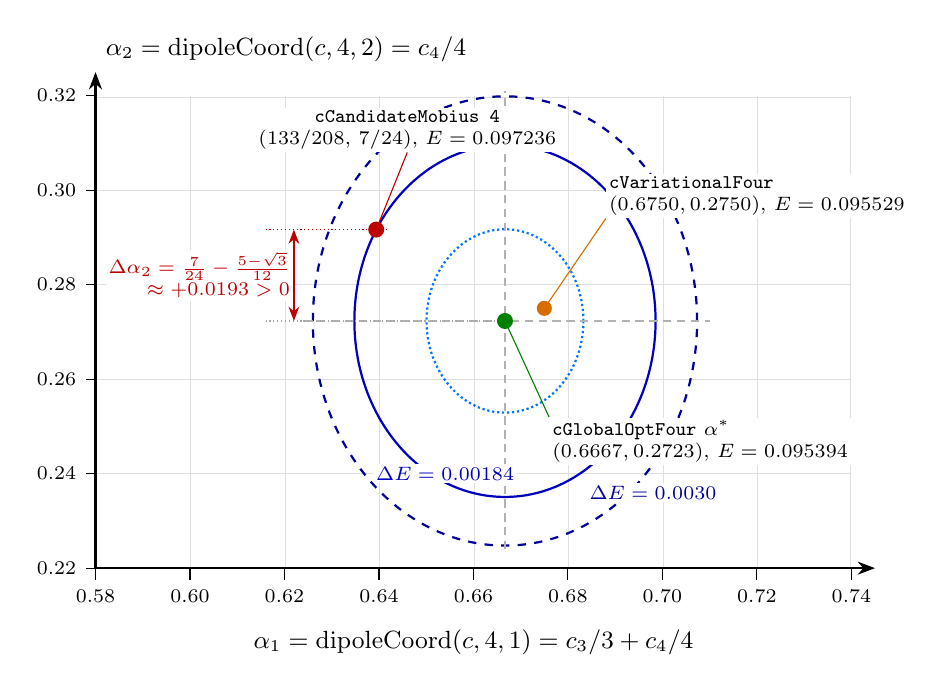
\begin{tikzpicture}[xscale=60, yscale=60]
  % Axes box: alpha1 in [0.58, 0.74], alpha2 in [0.22, 0.32]
  \draw[very thin, gray!25] (0.58,0.22) grid[xstep=0.02, ystep=0.02] (0.74,0.32);
  \draw[-{Stealth[length=2.2mm]}, thick] (0.58,0.22) -- (0.745,0.22);
  \node[below, font=\small] at (0.66, 0.209)
    {$\alpha_1 = \mathrm{dipoleCoord}(c, 4, 1) = c_3/3 + c_4/4$};
  \draw[-{Stealth[length=2.2mm]}, thick] (0.58,0.22) -- (0.58,0.325)
    node[above right, font=\small] {$\alpha_2 = \mathrm{dipoleCoord}(c, 4, 2) = c_4/4$};

  % Ticks
  \foreach \x in {0.58, 0.60, 0.62, 0.64, 0.66, 0.68, 0.70, 0.72, 0.74} {
    \draw (\x, 0.22) -- (\x, 0.2175) node[below, font=\scriptsize] {\x};
  }
  \foreach \y in {0.22, 0.24, 0.26, 0.28, 0.30, 0.32} {
    \draw (0.58, \y) -- (0.578, \y) node[left, font=\scriptsize] {\y};
  }

  % Axis-aligned orthogonal quadratic level sets centered at alpha* = (2/3, (5-sqrt(3))/12)
  % Delta E = (pi/sqrt(3))*(alpha1 - a1*)^2 + pi*(1 - 1/sqrt(3))*(alpha2 - a2*)^2
  % d = 0.0005, 0.001843 (Mobius contour), 0.0030
  \draw[blue!60!black, thick, dashed]
    (0.66667, 0.27233) ellipse [x radius=0.04067, y radius=0.04754];
  \draw[blue!75!black, thick]
    (0.66667, 0.27233) ellipse [x radius=0.03187, y radius=0.03725];
  \draw[blue!55!cyan, thick, densely dotted]
    (0.66667, 0.27233) ellipse [x radius=0.01660, y radius=0.01941];

  % Principal orthogonal dipole axes through alpha*
  \draw[gray!60, densely dashed] (0.624, 0.27233) -- (0.710, 0.27233);
  \draw[gray!60, densely dashed] (0.66667, 0.224) -- (0.66667, 0.321);

  % Vertical overshoot annotation at alpha1 = 133/208 = 0.63942
  \draw[red!70!black, thin, densely dotted] (0.616, 0.29167) -- (0.642, 0.29167);
  \draw[gray!70, thin, densely dotted] (0.616, 0.27233) -- (0.66667, 0.27233);
  \draw[{Stealth[length=1.8mm]}-{Stealth[length=1.8mm]}, red!75!black, thick]
    (0.622, 0.27233) -- (0.622, 0.29167)
    node[midway, left, font=\scriptsize, align=right, fill=white, inner sep=1pt]
    {$\Delta\alpha_2 = \frac{7}{24} - \frac{5-\sqrt{3}}{12}$\\$\approx +0.0193 > 0$};

  % Candidate points
  \fill[green!50!black] (0.66667, 0.27233) circle [radius=0.0017];
  \draw[green!50!black, thin] (0.66667, 0.27233) -- (0.676, 0.252)
    node[below right, font=\scriptsize, align=left, text=black, fill=white, inner sep=1pt]
    {\texttt{cGlobalOptFour} $\alpha^*$\\$(0.6667, 0.2723)$, $E = 0.095394$};

  \fill[orange!85!black] (0.67500, 0.27500) circle [radius=0.0016];
  \draw[orange!85!black, thin] (0.67500, 0.27500) -- (0.688, 0.294)
    node[above right, font=\scriptsize, align=left, text=black, fill=white, inner sep=1pt]
    {\texttt{cVariationalFour}\\$(0.6750, 0.2750)$, $E = 0.095529$};

  \fill[red!75!black] (0.63942, 0.29167) circle [radius=0.0017];
  \draw[red!75!black, thin] (0.63942, 0.29167) -- (0.646, 0.308)
    node[above, font=\scriptsize, align=center, text=black, fill=white, inner sep=1pt]
    {\texttt{cCandidateMobius 4}\\$(133/208,\, 7/24)$, $E = 0.097236$};

  % Contour labels
  \node[font=\scriptsize, text=blue!60!black, fill=white, inner sep=1pt]
    at (0.698, 0.236) {$\Delta E = 0.0030$};
  \node[font=\scriptsize, text=blue!75!black, fill=white, inner sep=1pt]
    at (0.654, 0.240) {$\Delta E = 0.00184$};
\end{tikzpicture}
\caption{Exact $2\mathrm{D}$ dipole phase portrait on $\mathcal{A}_4$ in coordinates $(\alpha_1, \alpha_2)$ (\texttt{UpstreamPR\_\allowbreak 4G} / \texttt{UpstreamPR\_\allowbreak 4L}). Because $d^{(1)} \perp d^{(2)}$ under $G_4^{(\mathrm{cot})}$ (\texttt{sum\_\allowbreak cumulative\allowbreak Dipole\_\allowbreak one\_\allowbreak two\_\allowbreak vasyunin\allowbreak GCot\_\allowbreak eq\_\allowbreak zero}), the iso-error contours are axis-aligned ellipses centered at the exact KKT optimum $\alpha^* = (\frac{2}{3}, \frac{5-\sqrt{3}}{12})$, with semi-axes scaled by $1/\sqrt{\pi/\sqrt{3}}$ horizontally and $1/\sqrt{\pi(1 - 1/\sqrt{3})}$ vertically. The vertical callout highlights the strict $k=4$ overshoot $\alpha_2(c_{\mathrm{opt}}^{(4)}) < \alpha_2(c_{\mathrm{mob}}^{(4)})$ (\texttt{dipole\allowbreak Coord\_\allowbreak cGlobal\allowbreak Opt\allowbreak Four\_\allowbreak two\_\allowbreak lt\_\allowbreak cCandidate\allowbreak Mobius\_\allowbreak four}).}
\label{fig:a4_phase_portrait}
\end{figure}

For general $N \ge 2$ (\texttt{UpstreamPR\_\allowbreak 4H\_\allowbreak Wavelet\allowbreak Rayleigh\allowbreak RHCriterion.lean}), the Rayleigh quotient $\mathcal{R}_{\mathrm{cot}}(h, N)$ is strictly scale-invariant ($\mathcal{R}_{\mathrm{cot}}(a h, N) = \mathcal{R}_{\mathrm{cot}}(h, N)$ for $a \ne 0$, \texttt{tangentRayleighQuotient\_\allowbreak smul}), arbitrary finite linear combinations of harmonic wavelets $h(k) = \sum_{m \in s} w_m w_k^{(m)}$ stay inside $\mathcal{A}_N^0$ (\texttt{sum\_\allowbreak smul\_\allowbreak harmonicWavelet\_\allowbreak mem\_\allowbreak tangent}) with $\mathcal{L}_{\mathrm{cot}}(h, N) = \sum_{m \in s} w_m \Delta^2 \delta_{\mathrm{cot}}(m)$ (\texttt{linearCotDrive\_\allowbreak sum\_\allowbreak harmonicWavelet\_\allowbreak eq}), and every $c \in \mathcal{A}_N$ projects cleanly onto the tangent shift $h_c = c - c_{\mathrm{anchor}} \in \mathcal{A}_N^0$ (\texttt{sub\_\allowbreak cBaseAnchor\_\allowbreak mem\_\allowbreak tangent}) with universal duality
\begin{equation}
S_{\mathrm{cot}}(c, N) \le \mathcal{R}_{\mathrm{cot}}(c - c_{\mathrm{anchor}}, N), \qquad 1 - \mathcal{R}_{\mathrm{cot}}(c - c_{\mathrm{anchor}}, N) \le \|1 - \textstyle\sum_{k=1}^N c_k \{1/(kx)\}\|_{L^2}^2
\end{equation}
(\texttt{SCot\_\allowbreak le\_\allowbreak tangent\allowbreak Rayleigh\allowbreak Quotient\_\allowbreak sub\_\allowbreak cBase\allowbreak Anchor}, \texttt{one\_\allowbreak sub\_\allowbreak tangent\allowbreak Rayleigh\allowbreak Quotient\_\allowbreak le\_\allowbreak l2\_\allowbreak dist}). Consequently, in \texttt{MathlibPR\_\allowbreak Forward\allowbreak Candidate.lean}, any family achieving $\sup_{h \in \mathcal{A}_N^0}\allowbreak \mathcal{R}_{\mathrm{cot}}(h, N)\allowbreak \to 1$ implies the Riemann Hypothesis (\texttt{riemann\allowbreak Hypothesis\_\allowbreak of\_\allowbreak tangent\allowbreak Rayleigh\allowbreak Quotient\_\allowbreak limit}).

Passing to the cumulative wavelet dipole basis $d^{(m)} := \sum_{r=1}^m w^{(r)}$ (\texttt{UpstreamPR\_\allowbreak 4I\_\allowbreak Cumulative\allowbreak Wavelet\allowbreak Dipole.lean}, \texttt{cumulative\allowbreak Dipole}, \texttt{cumulative\allowbreak Dipole\_\allowbreak mem\_\allowbreak tangent}) telescopes the second-difference cotangent stencil identically for all $N \ge m + 2$ into a pure boundary first difference (\texttt{linear\allowbreak Cot\allowbreak Drive\_\allowbreak cumulative\allowbreak Dipole\_\allowbreak eq}):
\begin{equation}
\mathcal{L}_{\mathrm{cot}}(d^{(m)}, N) = \delta_{\mathrm{cot}}(m + 2) - \delta_{\mathrm{cot}}(m + 1).
\end{equation}
At $N = 4$, $d^{(2)} = (1, -2, -3, 4)$ attains $Q_{\mathrm{cot}}(d^{(2)}, 4) = (1 - 1/\sqrt{3})\pi$ (\texttt{QCot\_\allowbreak cumulative\allowbreak Dipole\_\allowbreak two\_\allowbreak eq}) and exact orthogonality $d^{(1)} \perp d^{(2)}$ under $G_4^{(\mathrm{cot})}$ (\texttt{sum\_\allowbreak cumulative\allowbreak Dipole\_\allowbreak one\_\allowbreak two\_\allowbreak vasyunin\allowbreak GCot\_\allowbreak eq\_\allowbreak zero}); at $N = 5$, reciprocity cancellation $V(5, 1) + V(5, 4) = 0$ and $V(5, 2) + V(5, 3) = 0$ (\texttt{vasyunin\allowbreak Cot\allowbreak Sum\_\allowbreak five\_\allowbreak one\_\allowbreak add\_\allowbreak four}, \texttt{vasyunin\allowbreak Cot\allowbreak Sum\_\allowbreak five\_\allowbreak two\_\allowbreak add\_\allowbreak three}) proves $d^{(2)} \perp d^{(3)}$ under $G_5^{(\mathrm{cot})}$ algebraically without evaluating $\cot(\pi/5)$ (\texttt{sum\_\allowbreak cumulative\allowbreak Dipole\_\allowbreak two\_\allowbreak three\_\allowbreak vasyunin\allowbreak GCot\_\allowbreak five\_\allowbreak eq\_\allowbreak zero}).

Furthermore (\texttt{UpstreamPR\_\allowbreak 4J\_\allowbreak Four\allowbreak Point\allowbreak Dipole\allowbreak Kernel.lean}), pairing $d^{(m)}$ against any weighted sequence $F(k)/k$ collapses identically for all $N \ge m + 2$ to the 4-point functional $F(1) - F(2) - F(m+1) + F(m+2)$ (\texttt{cumulative\allowbreak Dipole\_\allowbreak div\_\allowbreak sum\_\allowbreak eq\_\allowbreak four\_\allowbreak point}). Via the unweighted symmetric cotangent kernel $K(j, k) := j k G_{j,k}^{(\mathrm{cot})}$ (\texttt{unweighted\allowbreak KCot}, \texttt{unweighted\allowbreak KCot\_\allowbreak comm}, \texttt{unweighted\allowbreak KCot\_\allowbreak diag}) and its boundary law $K(1, k) - K(2, k) = \frac{\pi}{2}\delta_{\mathrm{cot}}(k)$ (\texttt{unweighted\allowbreak KCot\_\allowbreak one\_\allowbreak sub\_\allowbreak two}), the entire $N \times N$ dipole Gram entry $\langle d^{(a)}, d^{(b)}\rangle_{G_N^{(\mathrm{cot})}}$ reduces to the $N$-independent 4-point local formula (\texttt{sum\_\allowbreak cumulative\allowbreak Dipole\_\allowbreak vasyunin\allowbreak GCot\_\allowbreak eq\_\allowbreak four\_\allowbreak point}):
\begin{multline}
\sum_{j=1}^N \sum_{k=1}^N d_j^{(a)} d_k^{(b)} G_{j,k}^{(\mathrm{cot})} = \frac{\pi}{2}\big(\delta_{\mathrm{cot}}(a+2) - \delta_{\mathrm{cot}}(a+1) + \delta_{\mathrm{cot}}(b+2) - \delta_{\mathrm{cot}}(b+1)\big) \\
+ K(a+1, b+1) - K(a+1, b+2) - K(a+2, b+1) + K(a+2, b+2).
\end{multline}
Figure~\ref{fig:stencil_telescoping} illustrates how the $3$-point harmonic stencil sums cleanly into the $4$-point boundary dipole.

\begin{figure}[htbp]
\centering
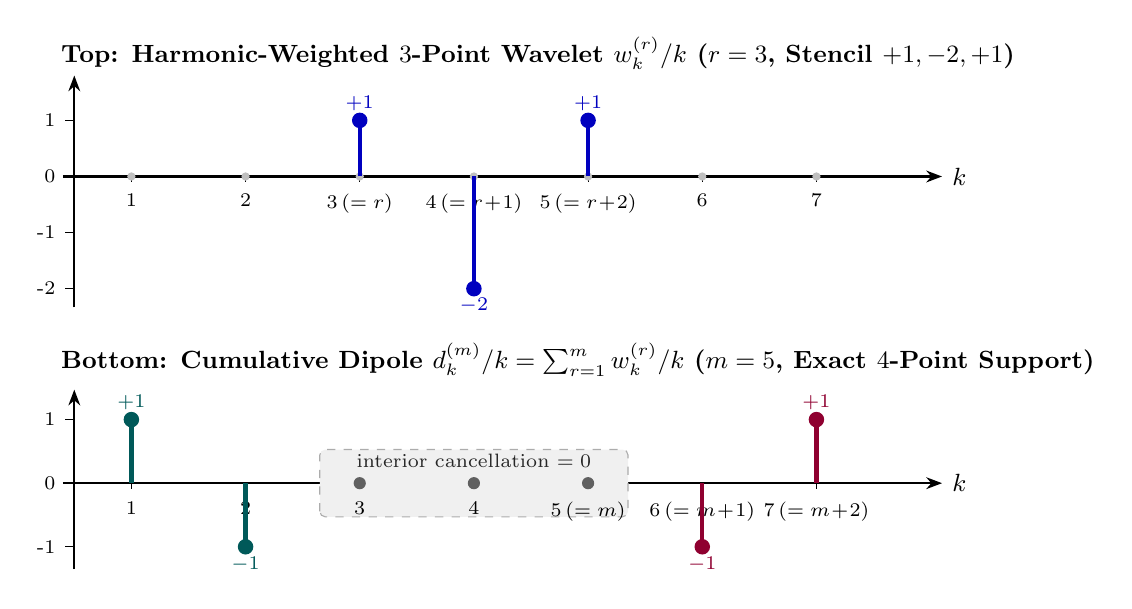
\begin{tikzpicture}[x=1.45cm, y=0.95cm]
  % Top Panel: 3-point harmonic-weighted wavelet w^(r)_k / k = (+1, -2, +1) at r = 3
  \node[anchor=west, font=\small\bfseries] at (0.3, 4.95)
    {Top: Harmonic-Weighted $3$-Point Wavelet $w^{(r)}_k / k$ ($r = 3$, Stencil $+1, -2, +1$)};
  \draw[-{Stealth[length=2mm]}, thick] (0.4, 3.3) -- (8.1, 3.3) node[right, font=\small] {$k$};
  \draw[-{Stealth[length=2mm]}, thick] (0.5, 1.55) -- (0.5, 4.65);
  \foreach \y in {-2, -1, 0, 1} {
    \draw (0.5, 3.3 + \y*0.75) -- (0.42, 3.3 + \y*0.75)
      node[left, font=\scriptsize] {\y};
  }
  \foreach \k in {1, 2, 3, 4, 5, 6, 7} {
    \draw (\k, 3.3) -- (\k, 3.22);
    \fill[gray!50] (\k, 3.3) circle (1.5pt);
  }
  \node[below, font=\scriptsize] at (1, 3.20) {$1$};
  \node[below, font=\scriptsize] at (2, 3.20) {$2$};
  \node[below, font=\scriptsize] at (3, 3.20) {$3\,(=r)$};
  \node[below, font=\scriptsize] at (4, 3.20) {$4\,(=r\!+\!1)$};
  \node[below, font=\scriptsize] at (5, 3.20) {$5\,(=r\!+\!2)$};
  \node[below, font=\scriptsize] at (6, 3.20) {$6$};
  \node[below, font=\scriptsize] at (7, 3.20) {$7$};

  % Stems at k = 3 (+1), 4 (-2), 5 (+1)
  \draw[blue!75!black, ultra thick] (3, 3.3) -- (3, 3.3 + 0.75);
  \fill[blue!75!black] (3, 3.3 + 0.75) circle (2.8pt)
    node[above, font=\scriptsize] {$+1$};
  \draw[blue!75!black, ultra thick] (4, 3.3) -- (4, 3.3 - 1.50);
  \fill[blue!75!black] (4, 3.3 - 1.50) circle (2.8pt)
    node[below, font=\scriptsize] {$-2$};
  \draw[blue!75!black, ultra thick] (5, 3.3) -- (5, 3.3 + 0.75);
  \fill[blue!75!black] (5, 3.3 + 0.75) circle (2.8pt)
    node[above, font=\scriptsize] {$+1$};

  % Bottom Panel: Cumulative Dipole d^(m)_k / k = (+1, -1, 0, ..., 0, -1, +1) for m = 5
  \node[anchor=west, font=\small\bfseries] at (0.3, 0.85)
    {Bottom: Cumulative Dipole $d^{(m)}_k / k = \sum_{r=1}^m w^{(r)}_k / k$ ($m = 5$, Exact $4$-Point Support)};
  \draw[-{Stealth[length=2mm]}, thick] (0.4, -0.8) -- (8.1, -0.8) node[right, font=\small] {$k$};
  \draw[-{Stealth[length=2mm]}, thick] (0.5, -1.95) -- (0.5, 0.45);
  \foreach \y in {-1, 0, 1} {
    \draw (0.5, -0.8 + \y*0.85) -- (0.42, -0.8 + \y*0.85)
      node[left, font=\scriptsize] {\y};
  }

  % Interior cancellation shaded region for k in {3, 4, 5}
  \fill[gray!12, rounded corners=2pt] (2.65, -1.25) rectangle (5.35, -0.35);
  \draw[gray!65, dashed, rounded corners=2pt] (2.65, -1.25) rectangle (5.35, -0.35);
  \node[font=\scriptsize, text=gray!30!black] at (4.0, -0.50) {interior cancellation $= 0$};

  \foreach \k in {1, 2, 3, 4, 5, 6, 7} {
    \draw (\k, -0.8) -- (\k, -0.88);
  }
  \foreach \k in {3, 4, 5} {
    \fill[gray!75!black] (\k, -0.8) circle (2.2pt);
  }
  \node[below, font=\scriptsize] at (1, -0.92) {$1$};
  \node[below, font=\scriptsize] at (2, -0.92) {$2$};
  \node[below, font=\scriptsize] at (3, -0.92) {$3$};
  \node[below, font=\scriptsize] at (4, -0.92) {$4$};
  \node[below, font=\scriptsize] at (5, -0.92) {$5\,(=m)$};
  \node[below, font=\scriptsize] at (6, -0.92) {$6\,(=m\!+\!1)$};
  \node[below, font=\scriptsize] at (7, -0.92) {$7\,(=m\!+\!2)$};

  % Surviving 4-point boundary spikes (+1, -1) at {1, 2} and (-1, +1) at {m+1, m+2}
  \draw[teal!70!black, ultra thick] (1, -0.8) -- (1, -0.8 + 0.85);
  \fill[teal!70!black] (1, -0.8 + 0.85) circle (2.8pt)
    node[above, font=\scriptsize] {$+1$};
  \draw[teal!70!black, ultra thick] (2, -0.8) -- (2, -0.8 - 0.85);
  \fill[teal!70!black] (2, -0.8 - 0.85) circle (2.8pt)
    node[below, font=\scriptsize] {$-1$};
  \draw[purple!75!black, ultra thick] (6, -0.8) -- (6, -0.8 - 0.85);
  \fill[purple!75!black] (6, -0.8 - 0.85) circle (2.8pt)
    node[below, font=\scriptsize] {$-1$};
  \draw[purple!75!black, ultra thick] (7, -0.8) -- (7, -0.8 + 0.85);
  \fill[purple!75!black] (7, -0.8 + 0.85) circle (2.8pt)
    node[above, font=\scriptsize] {$+1$};
\end{tikzpicture}
\caption{Top: $1/k$-weighted $3$-point harmonic wavelet $w^{(r)}_k / k = (+1, -2, +1)$ on $\{r, r+1, r+2\}$ (\texttt{harmonicWavelet\_div\_sum\_eq\_second\_diff}). Bottom: cumulative telescoping sum $d^{(m)}_k / k = \sum_{r=1}^m w^{(r)}_k / k$ collapses all interior weights on $3 \le k \le m$ identically to $0$, leaving only the fixed anchor dipole $(+1, -1)$ on $\{1, 2\}$ and the moving boundary dipole $(-1, +1)$ on $\{m+1, m+2\}$ (\texttt{cumulativeDipole\_eq\_four\_term} and \texttt{cumulativeDipole\_div\_sum\_eq\_four\_point}).}
\label{fig:stencil_telescoping}
\end{figure}

Finally (\texttt{UpstreamPR\_\allowbreak 4K\_\allowbreak General\allowbreak Wavelet\allowbreak Completeness.lean}), for every dimension $N \ge 2$, the $4$-term closed form of $d^{(m)}$ (\texttt{cumulative\allowbreak Dipole\_\allowbreak eq\_\allowbreak four\_\allowbreak term}) together with the suffix harmonic coordinates $\alpha_m(c) := \sum_{j=m+2}^N c_j / j$ (\texttt{dipole\allowbreak Coord}) and $\beta_r(c) := \sum_{m=r}^{N-2} \alpha_m(c)$ (\texttt{wavelet\allowbreak Coord}) proves unconditionally that $\{d^{(m)}\}_{m=1}^{N-2}$ and $\{w^{(r)}\}_{r=1}^{N-2}$ span the entire tangent hyperplane $\mathcal{A}_N^0$ and affine manifold $\mathcal{A}_N$ (\texttt{eq\_\allowbreak sum\_\allowbreak cumulative\allowbreak Dipole\_\allowbreak of\_\allowbreak mem\_\allowbreak tangent}, \texttt{eq\_\allowbreak sum\_\allowbreak harmonic\allowbreak Wavelet\_\allowbreak of\_\allowbreak mem\_\allowbreak tangent}, \texttt{eq\_\allowbreak cBase\allowbreak Anchor\_\allowbreak add\_\allowbreak sum\_\allowbreak cumulative\allowbreak Dipole\_\allowbreak of\_\allowbreak mem\_\allowbreak A\_\allowbreak N}, \texttt{eq\_\allowbreak cBase\allowbreak Anchor\_\allowbreak add\_\allowbreak sum\_\allowbreak harmonic\allowbreak Wavelet\_\allowbreak of\_\allowbreak mem\_\allowbreak A\_\allowbreak N}):
\begin{equation}
c_k = c_{\mathrm{anchor}, k} + \sum_{m=1}^{N-2} \alpha_m(c)\, d_k^{(m)} = c_{\mathrm{anchor}, k} + \sum_{r=1}^{N-2} \beta_r(c)\, w_k^{(r)} \qquad (1 \le k \le N).
\end{equation}
Combining general-$N$ wavelet tangent membership with the Rayleigh criterion in \texttt{MathlibPR\_\allowbreak Forward\allowbreak Candidate.lean} gives \texttt{riemann\allowbreak Hypothesis\_\allowbreak of\_\allowbreak wavelet\_\allowbreak rayleigh\_\allowbreak limit}: approaching Rayleigh quotient $1$ via finite linear combinations of $\{w^{(r)}\}_{r=1}^{N-2}$ implies the Riemann Hypothesis.

In \texttt{UpstreamPR\_\allowbreak 4L\_\allowbreak Dipole\allowbreak Quadratic\allowbreak Reduction.lean}, suffix--prefix duality collapses $\alpha_m(c)$ on $\{D_1(c, N) = 0\}$ to the negated prefix sum $\alpha_m(c) = -\sum_{j=1}^{m+1} c_j/j$ (\texttt{dipole\allowbreak Coord\_\allowbreak eq\_\allowbreak neg\_\allowbreak sum\_\allowbreak Icc\_\allowbreak of\_\allowbreak D1\_\allowbreak eq\_\allowbreak zero}). Defining the $N$-independent $4$-point dipole Gram entry $\widetilde{G}_{a,b}$ (\texttt{dipole\allowbreak Gram\allowbreak Entry}) reduces both $\mathcal{L}_{\mathrm{cot}}(h, N)$ and $Q_{\mathrm{cot}}(h, N)$ on $\mathcal{A}_N^0$ (\texttt{linear\allowbreak Cot\allowbreak Drive\_\allowbreak eq\_\allowbreak sum\_\allowbreak dipole\allowbreak Coord}, \texttt{QCot\_\allowbreak eq\_\allowbreak sum\_\allowbreak dipole\allowbreak Gram\allowbreak Entry}) and gives the master $N$-independent dipole quadratic form for every $c \in \mathcal{A}_N$ and $N \ge 2$ (\texttt{SCot\_\allowbreak eq\_\allowbreak dipole\allowbreak Coord\_\allowbreak quadratic\_\allowbreak of\_\allowbreak mem\_\allowbreak A\_\allowbreak N}):
\begin{equation}
S_{\mathrm{cot}}(c, N) = 2\pi \sum_{m=1}^{N-2} \alpha_m(c)\,\big(\delta_{\mathrm{cot}}(m+2) - \delta_{\mathrm{cot}}(m+1)\big) - \sum_{a=1}^{N-2}\sum_{b=1}^{N-2} \alpha_a(c)\,\alpha_b(c)\,\widetilde{G}_{a,b}.
\end{equation}
At $N = 4$, exact coordinate evaluation gives $(\alpha_1(c_{\mathrm{opt}}^{(4)}), \alpha_2(c_{\mathrm{opt}}^{(4)})) = (\tfrac{2}{3}, \tfrac{5-\sqrt{3}}{12})$ (\texttt{dipole\allowbreak Coord\_\allowbreak cGlobal\allowbreak Opt\allowbreak Four\_\allowbreak eval}) versus $(\alpha_1(c_{\mathrm{mob}}^{(4)}), \alpha_2(c_{\mathrm{mob}}^{(4)})) = (\tfrac{133}{208}, \tfrac{7}{24})$ (\texttt{dipole\allowbreak Coord\_\allowbreak cCandidate\allowbreak Mobius\_\allowbreak four\_\allowbreak eval}), certifying the strict $k = 4$ overshoot $\alpha_2(c_{\mathrm{opt}}^{(4)}) < \alpha_2(c_{\mathrm{mob}}^{(4)})$ (\texttt{dipole\allowbreak Coord\_\allowbreak cGlobal\allowbreak Opt\allowbreak Four\_\allowbreak two\_\allowbreak lt\_\allowbreak cCandidate\allowbreak Mobius\_\allowbreak four}).

Moreover (\texttt{UpstreamPR\_\allowbreak 4M\_\allowbreak Dipole\allowbreak Diagonal\allowbreak And\allowbreak Symmetry.lean}), the $4$-point dipole Gram kernel satisfies exact symmetry $\widetilde{G}_{a,b} = \widetilde{G}_{b,a}$ (\texttt{dipole\allowbreak Gram\allowbreak Entry\_\allowbreak comm}) and collapses on the diagonal $a = b = m$ to the single adjacent pair $(m+1, m+2)$ (\texttt{dipole\allowbreak Gram\allowbreak Entry\_\allowbreak diag\_\allowbreak eq}):
\begin{equation}
\widetilde{G}_{m,m} = \pi\big(\delta_{\mathrm{cot}}(m+2) - \delta_{\mathrm{cot}}(m+1)\big) - 2 K(m+1, m+2) \ge 0,
\end{equation}
where non-negativity for all $m \ge 1$ (\texttt{dipole\allowbreak Gram\allowbreak Entry\_\allowbreak diag\_\allowbreak nonneg}) follows unconditionally from $Q_{\mathrm{cot}}(d^{(m)}, N) = \widetilde{G}_{m,m}$ for all $N \ge m + 2$ (\texttt{QCot\_\allowbreak cumulative\allowbreak Dipole\_\allowbreak eq\_\allowbreak dipole\allowbreak Gram\allowbreak Entry\_\allowbreak diag}), with exact evaluations $\widetilde{G}_{1,1} = \pi/\sqrt{3}$, $\widetilde{G}_{2,2} = (1 - 1/\sqrt{3})\pi$, and $\widetilde{G}_{1,2} = 0$ (\texttt{dipole\allowbreak Gram\allowbreak Entry\_\allowbreak one\_\allowbreak one\_\allowbreak eq}, \texttt{dipole\allowbreak Gram\allowbreak Entry\_\allowbreak two\_\allowbreak two\_\allowbreak eq}, \texttt{dipole\allowbreak Gram\allowbreak Entry\_\allowbreak one\_\allowbreak two\_\allowbreak eq\_\allowbreak zero}).

\section{80-Digit Numerical Benchmarks and Spectral Obstructions}\label{sec:benchmark}

To probe convergence behavior beyond $N = 4$ without floating-point cancellation in the Vasyunin Gram matrix $G_N$ or the Lagrange multipliers~\eqref{eq:projectAffine}, the script \texttt{explore\_forward\_weights.py} evaluates seven candidate vectors across $N \in \{4, 8, 16, 32, 64, 128, 256\}$ using \texttt{mpmath} at $80$ decimal digits (\texttt{mp.dps = 80}). Five families come from projecting closed-form arithmetic seeds via \texttt{projectAffine} (Smooth Mollified M\"obius with $\alpha = 1, 2$; Logarithmic Riesz/Fej\'er $-\mu(k)\ln(N/k)/\ln N$; Harmonic M\"obius $-\mu(k)/k$; plus the two Clay--Galerkin single-ray variants with seeds $-\mu(k)/k$ and $-\mu(k)$), alongside the unconstrained KKT variational optimum on $\mathcal{A}_N$.

For every $N \in \{4, \dots, 256\}$, exact Cholesky factorization of $G_N$ succeeds (\texttt{cholesky\_spd = True}), with minimum Cholesky diagonal descending smoothly from $2.3285 \times 10^{-1}$ ($N=4$) to $7.1464 \times 10^{-3}$ ($N=256$). Agreement between the reduced and unreduced Vasyunin matrix formulas holds to $2.899 \times 10^{-81}$, affine defects $\max(|D_1|, |D_0 - 2|)$ are below $10^{-79}$, and $E(N) = 1 - S_{\mathrm{cot}}(c^{(N)}, N) > 0$ holds strictly in all runs. Table~\ref{tab:benchmark} summarizes the $80$-digit results.

\begin{table}[h!]
\centering
\scriptsize
\setlength{\tabcolsep}{3.2pt}
\begin{tabular}{@{}rccccccc@{}}
\toprule
$N$ & \textbf{Mobius} ($\alpha=1$) & \textbf{Mobius} ($\alpha=2$) & \textbf{Log Riesz} & \textbf{Harmonic} & \textbf{Clay-Gal.} ($-\mu/k$) & \textbf{Clay-Gal.} ($-\mu$) & \textbf{Var.\ Opt.} ($\mathcal{A}_N$) \\
\midrule
4   & 0.10082567 & 0.09723637 & 0.10417294 & 0.10218279 & 6.92525727 & 6.92525727 & 0.09539363 \\
8   & 0.02856641 & 0.04176774 & 0.03320549 & 0.03902275 & 0.24098566 & 0.15461919 & 0.02471483 \\
16  & 0.02194703 & 0.03463284 & 0.03357720 & 0.06656926 & 0.37938543 & 0.12345378 & 0.01795885 \\
32  & 0.01872208 & 0.02294467 & 0.03249525 & 0.10053985 & 0.04009097 & 0.07040140 & 0.01408463 \\
64  & 0.01532086 & 0.01630580 & 0.02849670 & 0.11659403 & 0.92700625 & 0.11516403 & 0.01139247 \\
128 & 0.01529665 & 0.01399341 & 0.02440191 & 0.12588183 & 0.09363099 & 0.23063618 & 0.00967077 \\
256 & 0.01479168 & 0.01321787 & 0.02009692 & 0.12847080 & 5.46178268 & 0.12081460 & 0.00824337 \\
\bottomrule
\end{tabular}
\caption{Continuous squared $L^2(0, 1)$ error $E(N) = 1 - S_{\mathrm{cot}}(c^{(N)}, N)$ computed at $80$ decimal digits on $\mathcal{A}_N$. The $\alpha=2$ column is precisely \texttt{cCandidateMobius N}.}
\label{tab:benchmark}
\end{table}

\subsection{Empirical Decay Fits and Two Analytic Spectral Obstructions}

Log-log and inverse-logarithmic regressions on the tail window $N \in [16, 256]$ reveal why no simple closed-form sequence yields fast convergence:
\begin{itemize}[noitemsep]
  \item \textbf{Variational Optimum:} Follows a logarithmic decay law, $E_{\mathrm{opt}}(N) \approx 0.05651 (\ln N)^{-1.12135}$ ($R^2_{\log} = 0.99976$ vs.\ $R^2_{\text{pow}} = 0.99092$), reaching $E_{\mathrm{opt}}(256) = 0.00824337$ with $S_{\mathrm{cot}} = 0.99175663$ and $\|c_{\mathrm{opt}}^{(256)}\|_2 = 5.0863$, whereas $c^{(N)}_{\mathrm{mob}}$ ($\alpha = 2$) reaches $E(256) = 0.01321787$ ($R^2_{\log} = 0.97998$ on $N = 4..256$).
  \item \textbf{Harmonic Saturation:} The fixed-weight harmonic family $-\mu(k)/k$ saturates in $\ell^2$-norm ($\|c^{(N)}\|_2 \approx 1.135$) and diverges away from $0$, worsening from $0.0390$ ($N=8$) to $0.1285$ ($N=256$).
\end{itemize}

This data isolates two fundamental spectral obstructions explaining why proving $\lim_{N\to\infty} E(N) = 0$ analytically remains open:
\begin{enumerate}[noitemsep]
  \item \textbf{Ill-Conditioning and Norm Growth (Twisted Fourth-Moment Barrier):} Direct spectral diagnostics show that the condition number $\kappa(G_N) = \lambda_{\max}(G_N)/\lambda_{\min}(G_N)$ grows superlinearly with $N$:
  \begin{gather}
  \kappa(G_4) = 30.75, \qquad \kappa(G_8) = 112.63, \qquad \kappa(G_{16}) = 544.35, \nonumber \\
  \kappa(G_{32}) = 2{,}726.05, \qquad \kappa(G_{64}) = 11{,}555.80.
  \end{gather}
  Driving $E(N) \to 0$ therefore forces $\|c^{(N)}\|_2 \to \infty$ (observed rising monotonically from $1.8734$ at $N=8$ to $5.0863$ at $N=256$ for the variational optimum, and to $5.6594$ for $\alpha = 2$ M\"obius). By Bettin--Conrey reciprocity~\cite{BettinConrey2013}, bounding $1 - S_{\mathrm{cot}}(c^{(N)}, N)$ as $\|c^{(N)}\|_2 \to \infty$ requires deep cancellation against the twisted fourth moment of $\zeta(1/2+it)$, which lies beyond known unconditional methods.
  \item \textbf{Rank-4 Clay Boundary Amplification:} In \texttt{clayGalerkinCandidate}, solving all four boundary equations $(D_0, D_0', D_1, D_1')$ simultaneously via the $4 \times 4$ boundary matrix $U_4$ (formalized in \texttt{Section8\_\allowbreak VasyuninBDR.lean} as \texttt{det\_U4\_eq\_log\_ratio}) produces
  \begin{equation}
  \det(U_4) = \frac{\ln 2}{24} \ln\!\left(\frac{256}{243}\right) \approx 0.00150517, \qquad \det(U_4)^{-1} \approx 664.38.
  \end{equation}
  This $664.38\times$ boundary amplification destabilizes unregularized 1-parameter rays along $U_4$ (explaining the oscillations $E(64) = 0.9270$, $E(256) = 5.4618$ for seed $-\mu(k)/k$), demonstrating why 2-constraint Lagrange projection \texttt{projectAffine} outperforms 4-constraint single-ray Galerkin updates at finite horizons.
\end{enumerate}

\begin{thebibliography}{9}
\raggedright

\bibitem{BaezDuarte2003}
L.~B\'aez-Duarte, \emph{A strengthening of the Nyman--Beurling criterion for the Riemann hypothesis}, Atti Accad. Naz. Lincei Cl. Sci. Fis. Mat. Natur. Rend. Lincei (9) Mat. Appl. \textbf{14} (2003), no.~1, 5--11.

\bibitem{BettinConrey2013}
S.~Bettin and J.~B.~Conrey, \emph{Period functions and cotangent sums}, Algebra \& Number Theory \textbf{7} (2013), no.~1, 215--242.

\bibitem{Mathlib}
The Mathlib Community, \emph{The Lean Mathematical Library}, \url{https://github.com/leanprover-community/mathlib4}, 2026.

\bibitem{Vasyunin1995}
V.~I.~Vasyunin, \emph{On a biorthogonal system related to the Riemann hypothesis}, Algebra i Analiz \textbf{7} (1995), no.~3, 118--135; English transl., St. Petersburg Math. J. \textbf{7} (1996), no.~3, 405--419.

\end{thebibliography}

\end{document}
